\PassOptionsToPackage{unicode}{hyperref}
\documentclass[aspectratio=1610, 9pt]{beamer}

% Load packages you need here
%\usepackage{polyglossia}
%\setmainlanguage{german}

\usepackage{csquotes}

\usepackage{subfigure}

\usepackage{amsmath}
\usepackage{amssymb}
\usepackage{mathtools}

\usepackage{braket}
\usepackage{graphicx}

\usepackage{booktabs}

\usepackage{hyperref}
\hypersetup{
  linkcolor= {tudark}, % internal links
  citecolor={tugreen}, % citations
  urlcolor={tudark} % external links/urls
  }
\usepackage{bookmark}

\usepackage[english]{babel}
\usepackage[
backend=biber,
style=authoryear-comp
]{biblatex}

\bibliography{lit.bib}

\usepackage{siunitx}
\usepackage{multicol}

\usepackage{booktabs}

\definecolor{light-gray}{HTML}{b0b5b0}

% load the theme after all packages

\usetheme[
  showtotalframes, % show total number of frames in the footline
]{tudo}

% Put settings here, like
\unimathsetup{
  math-style=ISO,
  bold-style=ISO,
  nabla=upright,
  partial=upright,
  mathrm=sym,
}

\title{Klassifikation von Tiergesichtern in drei Kategorien}
\author[T.~Magorsch,~J.~L.~Späh]{Tom Magorsch\\ Jan Lukas Späh}
\institute[ML-Seminar]{\\[0.3cm]TU Dortmund \\ \Large ML-Seminar}

\begin{document}



\maketitle

\begin{frame}{Datensatz und Fragestellung}
  \begin{columns}

    \column{0.8\textwidth}

    \begin{itemize}
    \item Quelle: \href{https://www.kaggle.com/andrewmvd/animal-faces?}{Kaggle}, Datensatz aus Dezember 2019 (\href{https://arxiv.org/abs/1912.01865}{arxiv:1912.01865}) mit \href{https://github.com/clovaai/stargan-v2}{Git-Repo}
    \item Lizenz: CreativeCommons (CC BY-NC 4.0)
    \item $16136$ Farbbilder verschiedener Tiere: $512\times 512$ Pixel
    \item Bilder in drei Kategorien aufgeteilt: (jeweils ca. 5000 Bilder)
      \begin{enumerate}
      \item Cat
      \item Dog
      \item Wildlife
      \end{enumerate}
    \item Datensatz bereits aufgeteilt in train (14633) und test (1503)
    \item Fragestellung der Klassifikation:\\
    \rightarrow{} ``Befindet sich auf dem Bild ein Hund, eine Katze oder etwas anderes?''
    \end{itemize}

    \column{0.2\textwidth}
    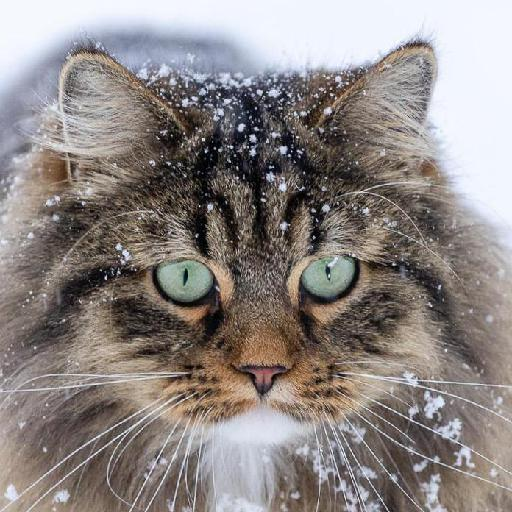
\includegraphics[scale=0.13]{images/cat.jpg}\\
    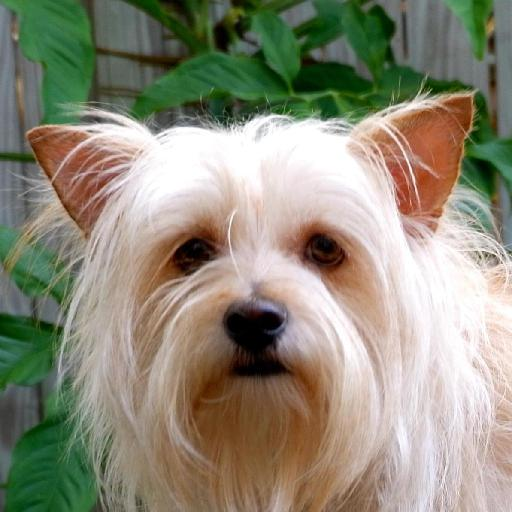
\includegraphics[scale=0.13]{images/dog.jpg}\\
    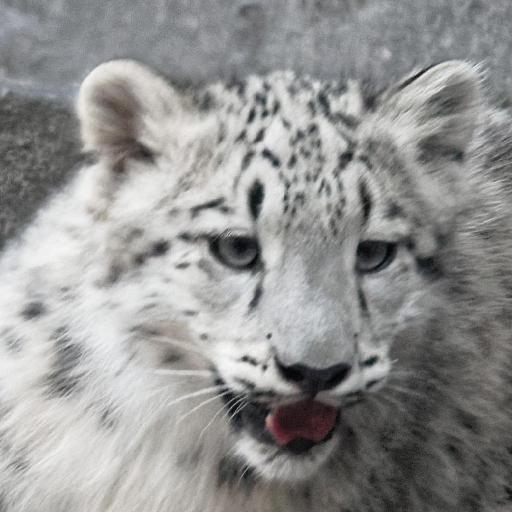
\includegraphics[scale=0.13]{images/wildlife.jpg}\\

  \end{columns}
\end{frame}

\begin{frame}{Alternativmethode}

  \begin{itemize}
    \item Methoden ohne Deep-Learning können meist schlecht mit reinen Pixeldaten umgehen\\
    \rightarrow{} Hochaufgelöster Datensatz: Bilder passen nicht ansatzweise in den RAM
    \begin{enumerate}
      \item 3D Colour Histograms: $512\times512\times3=786\,432 \to 8\times8\times8=512$ features
      \item PCA, die $95\%$ der Varianz erhält $\to 112$ features
      \item kNN-Klassifikation: Acc., Prec. und Rec. von $51$ bis $55$ Prozent
    \end{enumerate}
  \end{itemize}

  \begin{figure}
	   \centering
	   \subfigure{\label{fig:a}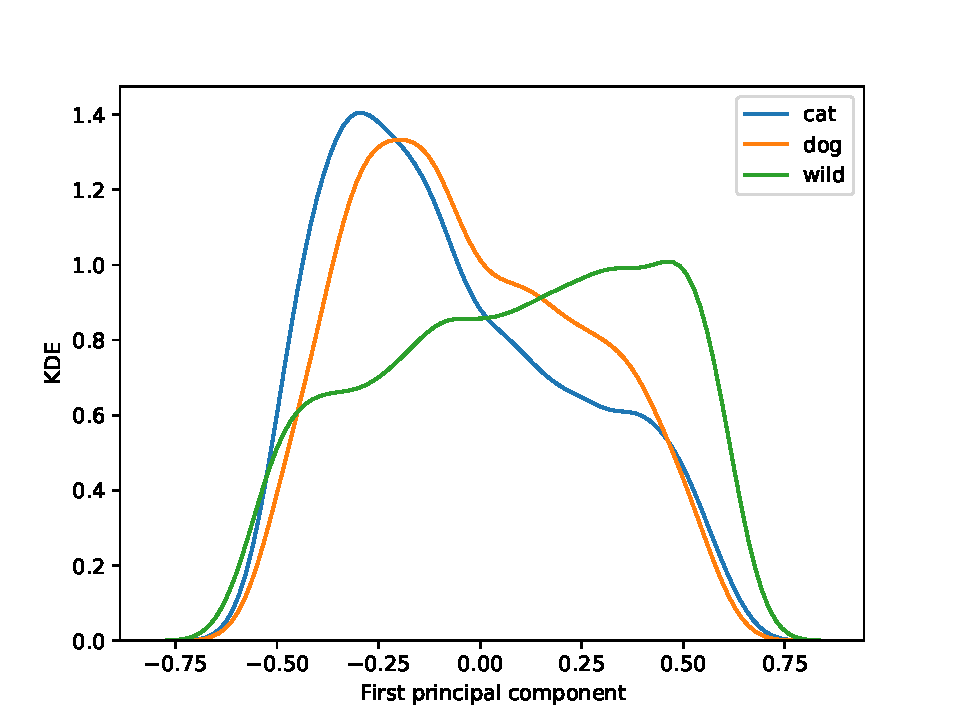
\includegraphics[width=60mm]{figures/kde_sns.pdf}}
	   \hspace{1cm}
	   \subfigure{\label{fig:b}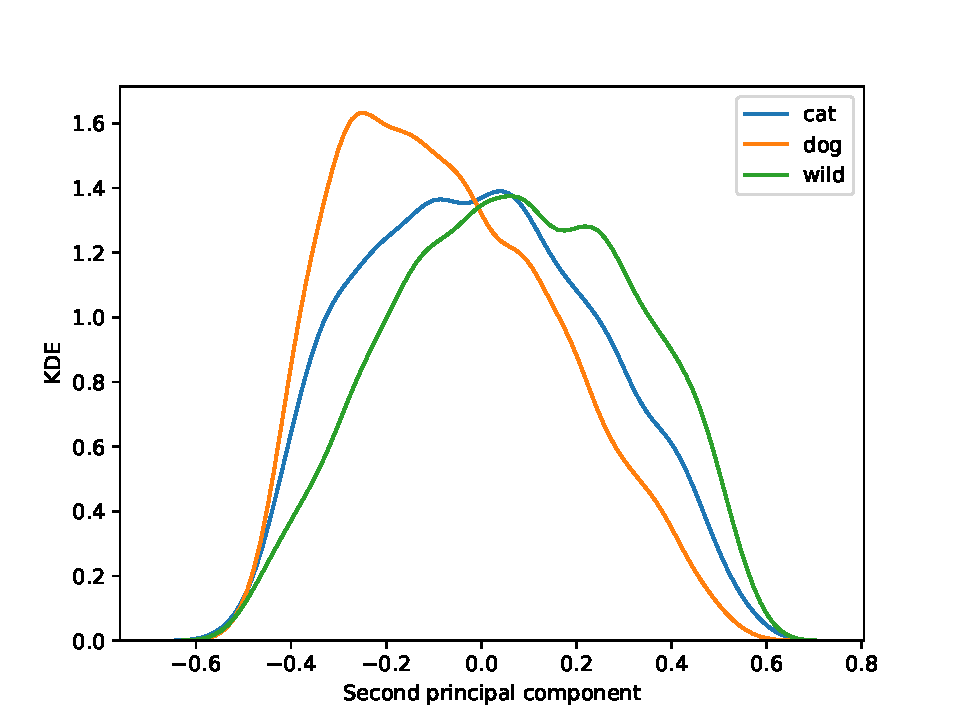
\includegraphics[width=60mm]{figures/kde_sns_2.pdf}}
  \end{figure}

\end{frame}

\begin{frame}{Optimierung zweier CNN}

  \begin{columns}
    \column{0.5\textwidth}
    \begin{itemize}
    \item Manuelles variieren der Netzwerkstruktur
      \begin{enumerate}
      \item Anzahl Convolutional Layer (1-6)
      \item Number Filters (16-128)
      \item Anzahl Dense Layer (1-4)
      \item Dense Units (16-128)
      \item Pooling size (2-5)
      \end{enumerate}
    \item Performance Unterschiede i.A. klein
    \item 2 Modelle ausgewählt die besonders gut waren
%      \begin{enumerate}
%      \item 5 Convolutional Layer, aufsteigende Filtersizes, ein Dense Layer - 128 Nodes
%      \item 2 Convolutional Layer, aufsteigende Filtersize, ein Dense Layer - 64 Nodes
%      \end{enumerate}
    \end{itemize}

    
    \column{0.5\textwidth}
    \begin{figure}
      \centering
      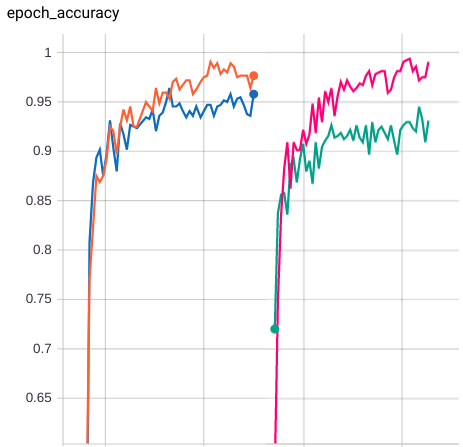
\includegraphics[scale=0.35]{images/models.png}      
      \caption{Links: 5 Convolutional Layer; Rechts: 2 Convolutional Layer; Die blaue und grüne Kurve zeigen die validation-accuracy, die orangene und magenta-farbene die trainings-accuracy.}
      \label{fig:acc}
    \end{figure}

  \end{columns}
\end{frame}



\begin{frame}
\begin{columns}

\column{0.3\textwidth}

\scalebox{0.73}{
\begin{tabular}{lll}
      \toprule
      Layer & Output Shape & Parameter\\
      \midrule
      Convolutional & (512, 512, 16) & 448 \\
      Max-Pooling & (256, 256, 16) & 0\\
      Convolutional & (254, 254, 32) & 4.640\\
      Max-Pooling & (127, 127, 32) & 0\\
      Convolutional & (125, 125, 64) & 18.496\\
      Max-Pooling & (62, 62, 64) & 0\\
      Convolutional & (60, 60, 96) & 55.392\\
      Max-Pooling & (30, 30, 96) & 0\\
      Convolutional & (28, 28, 96) & 83.040\\
      Max-Pooling & (14, 14, 96) & 0\\
      Flatten & (18.816) & 0\\
      Dense & (128) & 2.408.576\\
      Dense & (3) & 387\\
      \midrule
      Parameter & & 2.570.979\\
      \toprule
\end{tabular}
}


\scalebox{0.73}{
\begin{tabular}{lll}
      \toprule
      Layer & Output Shape & Parameter\\
      \midrule
      Convolutional & (512, 512, 16) & 448 \\
      Max-Pooling & (170, 170, 16) & 0\\
      Convolutional & (168, 168, 16) & 13.920\\
      Max-Pooling & (56, 56, 96) & 0\\
      Flatten & (301.056) & 0\\
      Dense & (64) & 19.267.648\\
      Dense & (3) & 195\\
      \midrule
      Parameter & & 19.282.211\\
      \toprule
\end{tabular}
}

\column{0.5\textwidth}

\begin{figure}
      \centering
      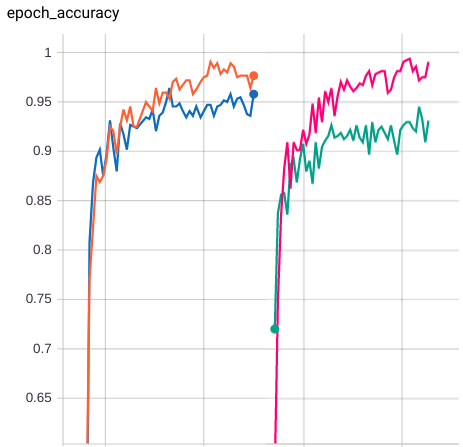
\includegraphics[scale=0.4]{images/models.png}     
      \caption{Links: 5 Convolutional Layer; Rechts: 2 Convolutional Layer; Die blaue und grüne Kurve zeigen die validation-accuracy, die orangene und magenta-farbene die trainings-accuracy.}
      \label{fig:acc}
    \end{figure}

\end{columns}

\end{frame}



\begin{frame}{Einfaches DNN}

  \centering
  \hspace{-1.3cm}\scalebox{1.6}{
  \begin{tabular}{lcccc}
    Pooling: & -  & 2x2  &  3x3  &  4x4\\
    Parameter: & 55.061.573  &  13.773.893  & 6.080.333  &  3.451.973\\
  \end{tabular}
  }

  \begin{figure}
    \centering
    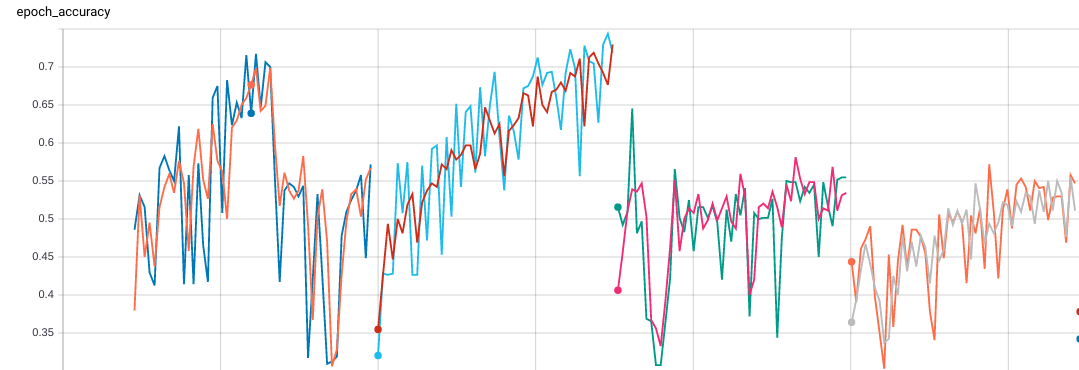
\includegraphics[scale=0.3]{images/dnn.png}
  \end{figure}
  
\end{frame}


\begin{frame}{Zusammenfassung}
  \begin{itemize}
  \item Alternativmethode KNN funktioniert besser als raten, jedoch keine hinreichend gute Klassifikation
  \item Einfaches DNN zu Viele Parameter, mit skalierten Daten bis zu 70\% Accuracy
  \item Convolutional Network funktioniert gut, mehrere Layer mit Pooling um Parameter zu reduzieren
  \item \textbf{Ausblick:} Regularisierung
  \end{itemize}
\end{frame}


%\begin{frame}{Methode zur Klassifikation und Vergleich mit Alternativen}
%  \begin{itemize}
%    \item Einfache Algorithmen sind kaum in der Lage, Bilder mit vergleichbarer Genauigkeit wie Deep-Learning-Methoden zu klassifizieren\\
%    \rightarrow{} Trainiere unterschiedliche neuronale Netze
%    \item Beispiel: Flaches NN, Tiefes NN und CNN
%    \item Mögliche einfache Vergleichsmethode für Bildklassifikation: z.B. kNN:
%    \begin{enumerate}
%      \item Extrahiere Features manuell aus den Bilder (z. B. Farbhistogram, Kontrast, Form-Features)
%      \item Definiere Metrik über dem Feature-Raum
%      \item Nutze Metrik für klassischen kNN
%    \end{enumerate}
%    \item Performance Measure für GAN: Kann ein DNN die generierten von den echten Bildern unterscheiden ?
%  \end{itemize}
%
%\end{frame}



\end{document}
